\documentclass[compress]{beamer}
\usecolortheme{default}

\usepackage{lmodern, epstopdf, multirow, array, setspace, bbm, tcolorbox, pbox, bm, mathtools, tikz}
\usepackage[T1]{fontenc}

\setbeamertemplate{frametitle}[default][center]
\setbeamertemplate{footline}{\hfill \insertframenumber/\inserttotalframenumber\hspace*{5pt}\vspace{5pt}}
\setbeamertemplate{navigation symbols}{}

\newlength{\wideitemsep}
\setlength{\wideitemsep}{\itemsep}
\addtolength{\wideitemsep}{4pt}
\let\olditem\item
\renewcommand{\item}{\setlength{\itemsep}{\wideitemsep}\olditem}
\setlength{\leftmargini}{12pt}
\setlength{\leftmarginii}{14pt}
\setbeamertemplate{itemize/enumerate subbody begin}{\vspace{6pt}}
\setbeamertemplate{itemize item}[circle]
\setbeamertemplate{enumerate item}[circle]
\setbeamertemplate{enumerate subitem}[default]

\setbeamercolor{alerted text}{fg=blue}
\setbeamersize{text margin left=1.5em,text margin right=1.5em}

\tcbset{
    colback=white,
    colframe=black,
    coltext=black,
    coltitle=blue,
    colbacktitle=white,
    boxrule=1pt,
    titlerule=0pt,
    toptitle=4pt,
    top=2pt
}

\newenvironment{changemargin}[2]{% 
  \begin{list}{}{% 
    \setlength{\topsep}{0pt}% 
    \setlength{\leftmargin}{#1}% 
    \setlength{\rightmargin}{#2}% 
    \setlength{\listparindent}{\parindent}% 
    \setlength{\itemindent}{\parindent}% 
    \setlength{\parsep}{\parskip}% 
  }% 
  \item[]}{\end{list}}
  
\newenvironment{defn}{%
  \begin{tcolorbox}[title={Definition}]%
  }{\end{tcolorbox}}
  
\newenvironment{prop}[1]{%
  \begin{tcolorbox}[title={Proposition #1}]%
  }{\end{tcolorbox}}
  
\newcommand{\cit}[1]{{\footnotesize \textcolor[rgb]{0.5,0,0}{#1}}}

% Font size for code listings (verbatim blocks); reset with \normalsize
\newcommand{\codesize}{\fontsize{7}{8.5}\selectfont}

\newcommand{\slidesetup}[1]{%
  \title{#1}%
  \subtitle{\texorpdfstring{\vspace{0.3\baselineskip}}{} {\small This version: \today}}%
  \author[Mikkel Plagborg-Moller]{ECMA 31150, Spring 2026 \texorpdfstring{\\[0.5ex]}{} University of Chicago \texorpdfstring{\\[0.5ex]}{} Department of Economics \texorpdfstring{\\[4ex]}{} Mikkel Plagborg-Moller}%
  \date{}%
}

% \circleoverlay[options]{text}
% Draws a red circle with a text box nearby on a tikz overlay.
% Options (with defaults):
%   cx=0cm, cy=0cm      - circle center (shift from page center)
%   r=1cm               - circle radius
%   tx=0cm, ty=0cm      - text box offset from circle center
%   text anchor=east    - anchor of text node (east = text left, west = text right)
%   font=\normalsize    - font size for text
\pgfkeys{
  /circleoverlay/.cd,
  cx/.store in=\cocx, cx=0cm,
  cy/.store in=\cocy, cy=0cm,
  r/.store in=\cor, r=1cm,
  tx/.store in=\cotx, tx=0cm,
  ty/.store in=\coty, ty=0cm,
  text anchor/.store in=\cotextanchor, text anchor=east,
  font/.store in=\cofont, font=\normalsize,
}
\newcommand{\circleoverlay}[2][]{%
  \pgfkeys{/circleoverlay/.cd, cx=0cm, cy=0cm, r=1cm, tx=0cm, ty=0cm, text anchor=east, font=\normalsize, #1}%
  \pgfmathsetlengthmacro{\circlediameter}{2*\cor}%
  \node[draw=red, line width=2pt, circle, minimum size=\circlediameter, inner sep=0pt]
    (tmpcirc) at ([xshift=\cocx,yshift=\cocy]current page.center) {};%
  \node[anchor=\cotextanchor, fill=white, draw=red, text=red, inner sep=4pt, align=left, font=\cofont]
    at ([xshift=\cotx,yshift=\coty]tmpcirc.center) {#2};%
}

\DeclareMathOperator*{\argmax}{argmax}
\DeclareMathOperator*{\argmin}{argmin}
\DeclareMathOperator{\diag}{diag}
\DeclareMathOperator{\var}{Var}
\DeclareMathOperator{\cov}{Cov}
\DeclareMathOperator{\corr}{Corr}
\DeclareMathOperator{\lrv}{LRV}


\slidesetup{Forecasting with stationary models III}

\begin{document}
\frame{
\maketitle
}

\frame{
\frametitle{Plan for this slide deck}
\begin{enumerate}
\item Sources of forecast errors
\item Forecast evaluation
\item Forecast intervals
\end{enumerate}
}

\frame{
\frametitle{Feasible AR forecast}
\[y_t = c + a_1 y_{t-1} + a_2 y_{t-2} + \dots + a_p y_{t-p} + u_t,\quad E[u_t \mid \lbrace y_s \rbrace_{s<t}]=0\]
\begin{itemize}
\item We've discussed the optimal one-step-ahead forecast:
\[y_{T+1|T} = c + a_1 y_T + \dots + a_p y_{T-p+1}.\]
\item In practice, we don't know the parameters, so we substitute the OLS estimates. This yields a feasible forecast:
\[\hat{y}_{T+1|T} \equiv \hat{c} + \hat{a}_1 y_T + \dots + \hat{a}_p y_{T-p+1}.\]
\end{itemize}
}

\frame{
\frametitle{Forecast error}
\begin{itemize}
\item Our forecast is never going to be exactly right.
\item According to the model, the \textbf{forecast error} equals
\[y_{T+1}-\hat{y}_{T+1|T} = (c-\hat{c}) + (a_1-\hat{a}_1)y_T + \dots + (a_p-\hat{a}_p)y_{T-p+1} + u_{T+1}.\]
\item The last term is the shock at time $T+1$. The uncertainty about this term never goes away, even if $T$ is large.
\item The other terms are due to estimation errors in the parameters. These errors vanish as the sample size $T$ gets large.
\item Of course, another source of error is model misspecification: it could be wrong to assume that $y_{T+1}$ satisfies an AR($p$) equation.
\begin{itemize}
\item $p$ too small, non-linearities, structural breaks\dots
\end{itemize}
\end{itemize}
}

\frame{
\frametitle{Forecast quality}
\begin{itemize}
\item A common way to measure the quality of a forecast $\hat{y}_{T+1|T}$ is the \textbf{mean-squared forecast error} (MSFE):
\[\mathit{MSFE} \equiv E[(y_{T+1}-\hat{y}_{T+1|T})^2].\]
\item If we take the square root, we get the \textbf{root MSFE} (RMSFE):
\[\mathit{RMSFE} \equiv \sqrt{E[(y_{T+1}-\hat{y}_{T+1|T})^2]}.\]
\item Of course, we could define similar concepts for multi-step forecasts:
\[\mathit{MSFE}(h) \equiv E[(y_{T+h}-\hat{y}_{T+h|T})^2].\]
\end{itemize}
}

\frame{
\frametitle{Forecast evaluation}
\begin{itemize}
\item How do we estimate the MSFE in the data?
\item This is typically done through \textbf{recursive pseudo-out-of-sample forecasting}:
\begin{enumerate}
\item First estimate the model using data only up to some time $\underline{t}$ in the past (e.g., 1947Q1--1969Q4). Then forecast the $\underline{t}+1$ observation (1970Q1). Compute the forecast error $\hat{e}_{\underline{t}+1|\underline{t}}$.
\item Now \emph{re-estimate} the model using data up to time $\underline{t}+1$ (1970Q1). Forecast the $\underline{t}+2$ observation (1970Q2) and compute forecast error $\hat{e}_{\underline{t}+2|\underline{t}+1}$.
\item Etc. Stop at time $T$ when we run out of data.
\item We now have $T-\underline{t}$ forecast errors through time. Estimate the MSFE as
\[\widehat{\mathit{MSFE}} \equiv \frac{1}{T-\underline{t}}\sum_{t=\underline{t}}^{T-1} \hat{e}_{t+1|t}^2.\]
\end{enumerate}
\end{itemize}
}

\frame{
\frametitle{Comparing forecast methods}
\begin{itemize}
\item The procedure on the previous slide uses real data, so does not assume that any particular model is the correct one that generated the data.
\item Thus, if we are wondering which of several forecast methods to use, we can estimate their respective MSFEs as on the previous slide. Then pick the method with the lowest MSFE.
\end{itemize}
}

\frame{
\frametitle{Comparing forecast methods: example}
\begin{itemize}
\item Example: recursive evaluation of CPI inflation forecasts.
\item Two competing methods: AR(4) vs.\ no-change forecast ($y_{t+1|t}=y_t$).
\item We start the evaluation in January 1970, using data back to 1947 to estimate the AR model.
\item Estimated RMSFE for AR(4): $0.250$
\item Estimated RMSFE for no-change forecast: $0.279$
\item For comparison, the sample std.\ dev.\ of month-over-month inflation is 0.340.
\end{itemize}
}

\frame{
\begin{figure}
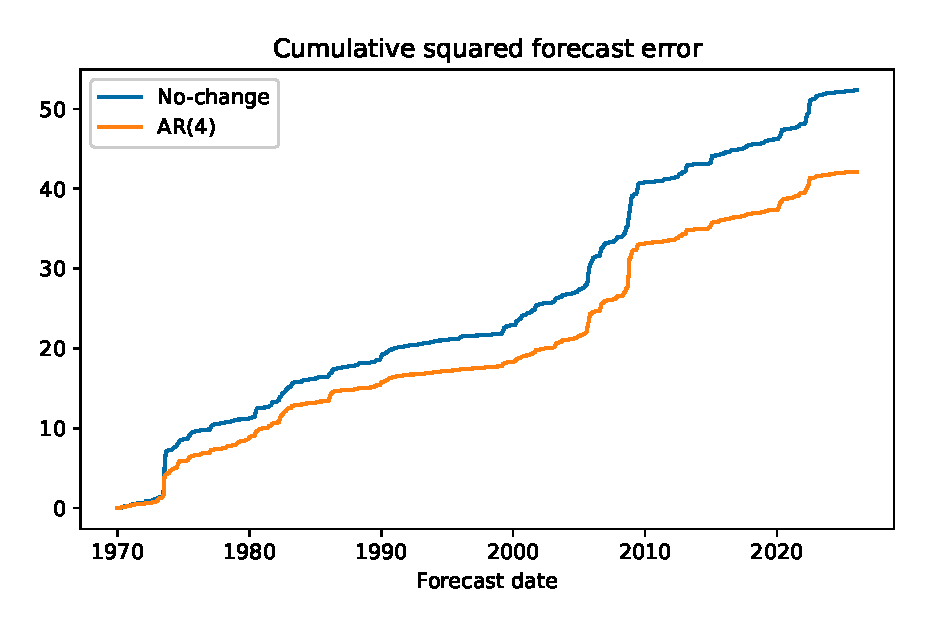
\includegraphics[width=0.9\linewidth]{fig/sfe.eps}
\end{figure}
}

\frame{
\frametitle{Extensions}
\begin{itemize}
\item Alternative to MSFE: \textbf{mean absolute forecast error}
\[\mathit{MAFE} \equiv E[|y_{T+1}-\hat{y}_{T+1|T}|].\]
Less sensitive to a few large forecast errors.
\item The recursive pseudo-out-of-sample approach can easily be applied to multi-step forecasts, too.
\item Both MSFE and MAFE give equal weight to positive and negative forecast errors. In some settings we may wish to weight over-predictions and under-predictions differently.
\item If we're worried about structural breaks, we can estimate the model on a fixed sample size $T_\text{window}$ at all time points, e.g., 20 years. This is called \textbf{rolling window} pseudo-out-of-sample evaluation.
\end{itemize}
}

\frame{
\frametitle{Forecast interval}
\begin{itemize}
\item So far we've produced \textbf{point forecasts}: a single ``best guess'' for what the future value of the time series will be.
\item But these point forecasts will be associated with substantial uncertainty. The RMSFE is one measure of this uncertainty.
\item In analogy with confidence intervals for parameters, we would like a \textbf{forecast interval} $\hat{\mathcal{I}}_{T+1|T}$ with the property
\[P(y_{T+1} \in \hat{\mathcal{I}}_{T+1|T}) \approx 1-\alpha,\]
for some pre-specified coverage probability $1-\alpha$.
\end{itemize}
}

\frame{
\frametitle{Distribution of forecast error}
\begin{itemize}
\item Let's go back to our model-implied forecast error
\[y_{T+1}-\hat{y}_{T+1|T} = (c-\hat{c}) + (a_1-\hat{a}_1)y_T + \dots + (a_p-\hat{a}_p)y_{T-p+1} + u_{T+1}.\]
\item Now make the (strong) assumption that the shocks are i.i.d.\ normally distributed: $u_t \overset{iid}{\sim} N(0,\sigma_u^2)$.
\item Recall that when $T$ is large, parameter estimation errors are negligible relative to $\sigma_u^2 \equiv \var(u_{T+1})$.
\begin{itemize}
\item We will later learn how to also take parameter uncertainty into account using Bayesian methods.
\end{itemize}
\item Hence, as $T \to \infty$,
\[y_{T+1}-\hat{y}_{T+1|T} \overset{approx}{\sim} N\big(0, \underbrace{\mathit{MSFE}}_{\approx \sigma_u^2} \big).\]
\end{itemize}
}

\frame{
\frametitle{Forecast interval: construction}
\begin{itemize}
\item Given an estimate $\widehat{\mathit{RMSFE}}$ of $\sqrt{\mathit{MSFE}}$, we have
\[\frac{y_{T+1}-\hat{y}_{T+1|T}}{\widehat{\mathit{RMSFE}}} \overset{approx}{\sim} N(0,1).\]
\item Let $Q_{1-\alpha/2}$ be the $1-\alpha/2$ quantile of the standard normal distribution ($\approx 1.96$ for $\alpha=0.05$).
\item Then
\[P\left(y_{T+1} \in \hat{\mathcal{I}}_{T+1|T}\right) \approx 1-\alpha,\quad \text{where}\]
{\footnotesize
\[\boxed{\hat{\mathcal{I}}_{T+1|T} \equiv \left[\hat{y}_{T+1|T} - Q_{1-\alpha/2}\widehat{\mathit{RMSFE}}, \hat{y}_{T+1|T} + Q_{1-\alpha/2}\widehat{\mathit{RMSFE}}\right]}.\]
}
\item Note: we're relying heavily on the assumption that the shock $u_{T+1}$ is normally distributed. This is \emph{not} a consequence of a CLT.
\end{itemize}
}

\frame{
\frametitle{Forecast interval: estimating the RMSFE}
\begin{itemize}
\item Two ways of obtaining an estimate $\widehat{\mathit{RMSFE}}$:
\begin{enumerate}
\item Pseudo-out-of-sample forecasting.
\item Model-based: $\widehat{\mathit{RMSFE}} = \sqrt{\hat{\sigma}_u^2}$ from the AR regression output.
\end{enumerate}
\end{itemize}
}



\frame{
\frametitle{Forecast interval: evaluation}
\begin{itemize}
\item How do we evaluate the quality of a forecast interval?
\item Using the pseudo-out-of-sample procedure, we can compute the fraction of the forecast intervals $\hat{\mathcal{I}}_{t+1|t}$ (constructed at each point in time) that actually cover their respective realized values $y_{t+1}$. This empirical coverage rate should be close to $1-\alpha$.
\begin{itemize}
\item Can use this to evaluate the assumption of normal shocks.
\end{itemize}
\item Subject to having accurate coverage, we prefer forecast intervals that tend to be narrow. Can compute the average length of the intervals in the pseudo-out-of-sample evaluation.
\end{itemize}
}

\frame{
\begin{figure}
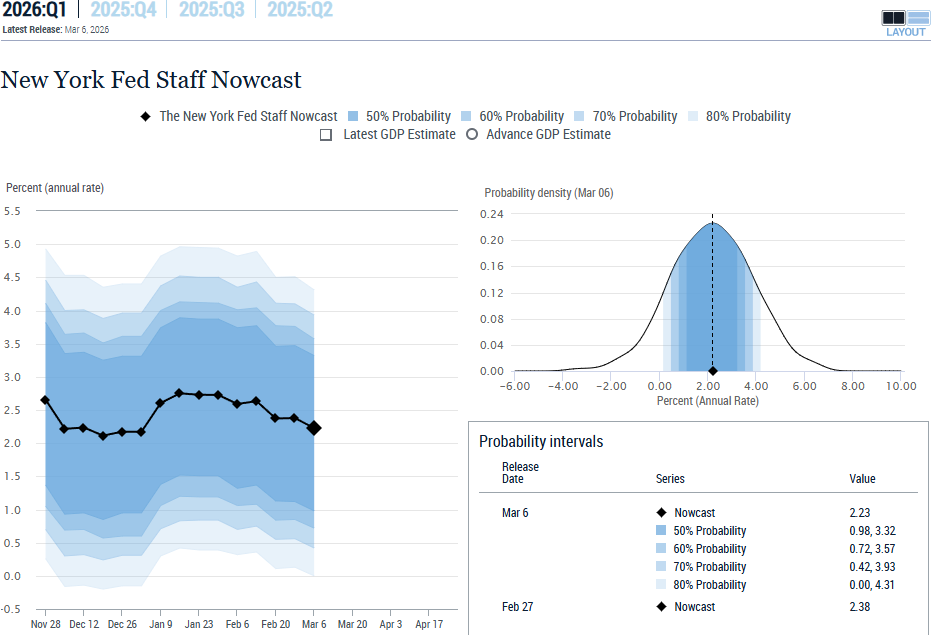
\includegraphics[width=\linewidth]{fig/nyfed_nowcast1.png}
\end{figure}
}

\frame{
\frametitle{Direct vs.\ iterated multi-step forecasts}
\begin{itemize}
\item Recall: $h$-step forecast in AR(1) model:
\[\hat{y}_{T+h|T} = \hat{\rho}^h y_T + \frac{1-\hat{\rho}^h}{1-\hat{\rho}}\hat{c}.\]
This is an \textbf{iterated} multi-step forecast, as it's obtained by iterating on the recursive AR model.
\item Alternative approach: \textbf{direct} multi-step forecast regression
\[y_{t+h} = \hat{\beta}_0 + \hat{\beta}_1y_t + \hat{v}_{t+h},\]
yielding $h$-step forecast $\hat{y}_{T+h|T}^\text{direct} \equiv \hat{\beta}_0 + \hat{\beta}_1 y_T$.
\item Direct forecasts are less subject to model misspecification bias, as they do not impose a recursive functional form.
\item But their variance is higher. Typically $\mathit{MSFE}_\text{direct}>\mathit{MSFE}_\text{iterated}$.
\end{itemize}
}

\frame{
\frametitle{What did we learn?}
\begin{itemize}
\item Sources of forecast errors:
\begin{enumerate}
\item Parameter uncertainty
\item Unforecastable shock
\item Model misspecification
\end{enumerate}
\item Forecast evaluation
\begin{itemize}
\item (R)MSFE
\item Recursive pseudo-out-of-sample forecasts
\end{itemize}
\item Forecast interval, assuming normally distributed shocks
\item Direct vs.\ iterated multi-step forecasts
\end{itemize}
}

\frame{
\frametitle{Looking ahead}
\begin{itemize}
\item Allowing for richer time series dynamics
\begin{itemize}
\item Moving averages
\item ARMA models
\end{itemize}
\item Lag polynomials to facilitate analysis of rich time series models
\item When is the AR($p$) model stationary?
\end{itemize}
}

\end{document}
